\documentclass[11pt]{amsart}
\usepackage{alttpreamble}
% \usepackage{tocloft}
% \renewcommand{\cftsecleader}{\cftdotfill{\cftdotsep}}
\begin{document}
\author{Maya Basu}
\author{Ethan Clayton}
\author{Fredrick Mooers}

\address{University of California, Berkeley}
\email{mab@berkeley.edu}

\address{University of Illinois, Urbana-Champaign}
\email{ewc3@illinois.edu}

\address{Virginia Tech}
\email{mooersfl24@vt.edu}

\title{Persistent Legendrian contact homology in $\R^3$}



\subjclass{53D42; 53D10, 57K10; 55N31}
\keywords{Legendrian contact homology, Legendrian knot, Persistent Homology}

\maketitle

\tableofcontents
\newpage

\section{June 17th: Flooding the Knot}



\begin{definition}[Knot Chart]
    Consider a set of inequalities generated by considering area loops. Picking this collection of inequalities so that the entire knot is covered by area loops, and so that these area loops are of minimal size, we obtain a knot chart.
\end{definition}

\subsection{Algebraic Description}
Consider the set of all inequalities obtained by creating a chart for the knot. Follow the following procedure:

\begin{enumerate}
    \item Set $n = 1$
    \item Considering the (finite) collection of inequalities in the knot chart, find the generators $g_1 \cdots g_k$ which are only listed as positive terms in every inequality.
    \item Assign generators $g_1 \cdots g_k$ to tier $n$.
    \item Delete every inequality in the knot chart which contains at least one copy of any of the generators $g_1 \cdots g_k$.
    \item Incriment $n$ by $1$, and start from step $2$, untill the knot map is empty
    \item The remaining generators are placed in the "extras" tier
\end{enumerate}


\subsection{Geometric Description}

Consider the set of all loops which are described by an inequality in the knot diagram. Label each corner of an intersection as $+$ or $-$ as wether traversing the intersection CCW increases or decreases the $z$ value.


\begin{enumerate}
    \item Set $n = 1$
    \item Consider every generator $g_1 \cdots g_k$ where every negative corner of the crossing is in a shaded region. 
    \item Assign generators $g_1 \cdots g_k$ to tier $n$.
    \item Shade in ("flood") each region which is an area loop including these generators
    \item Incriment $n$ by $1$, and start from step $2$, untill the knot is completly flooded.
    \item The remaining generators are placed in the "extras" tier

\end{enumerate}

The following is an example with the Chekanov knot, flooded with increasingly lighter tiers:


\begin{figure}[htbp]
  \centering
  \includesvg{CE2.svg}
  \caption{Flood}
\end{figure}


\subsection{Observations}





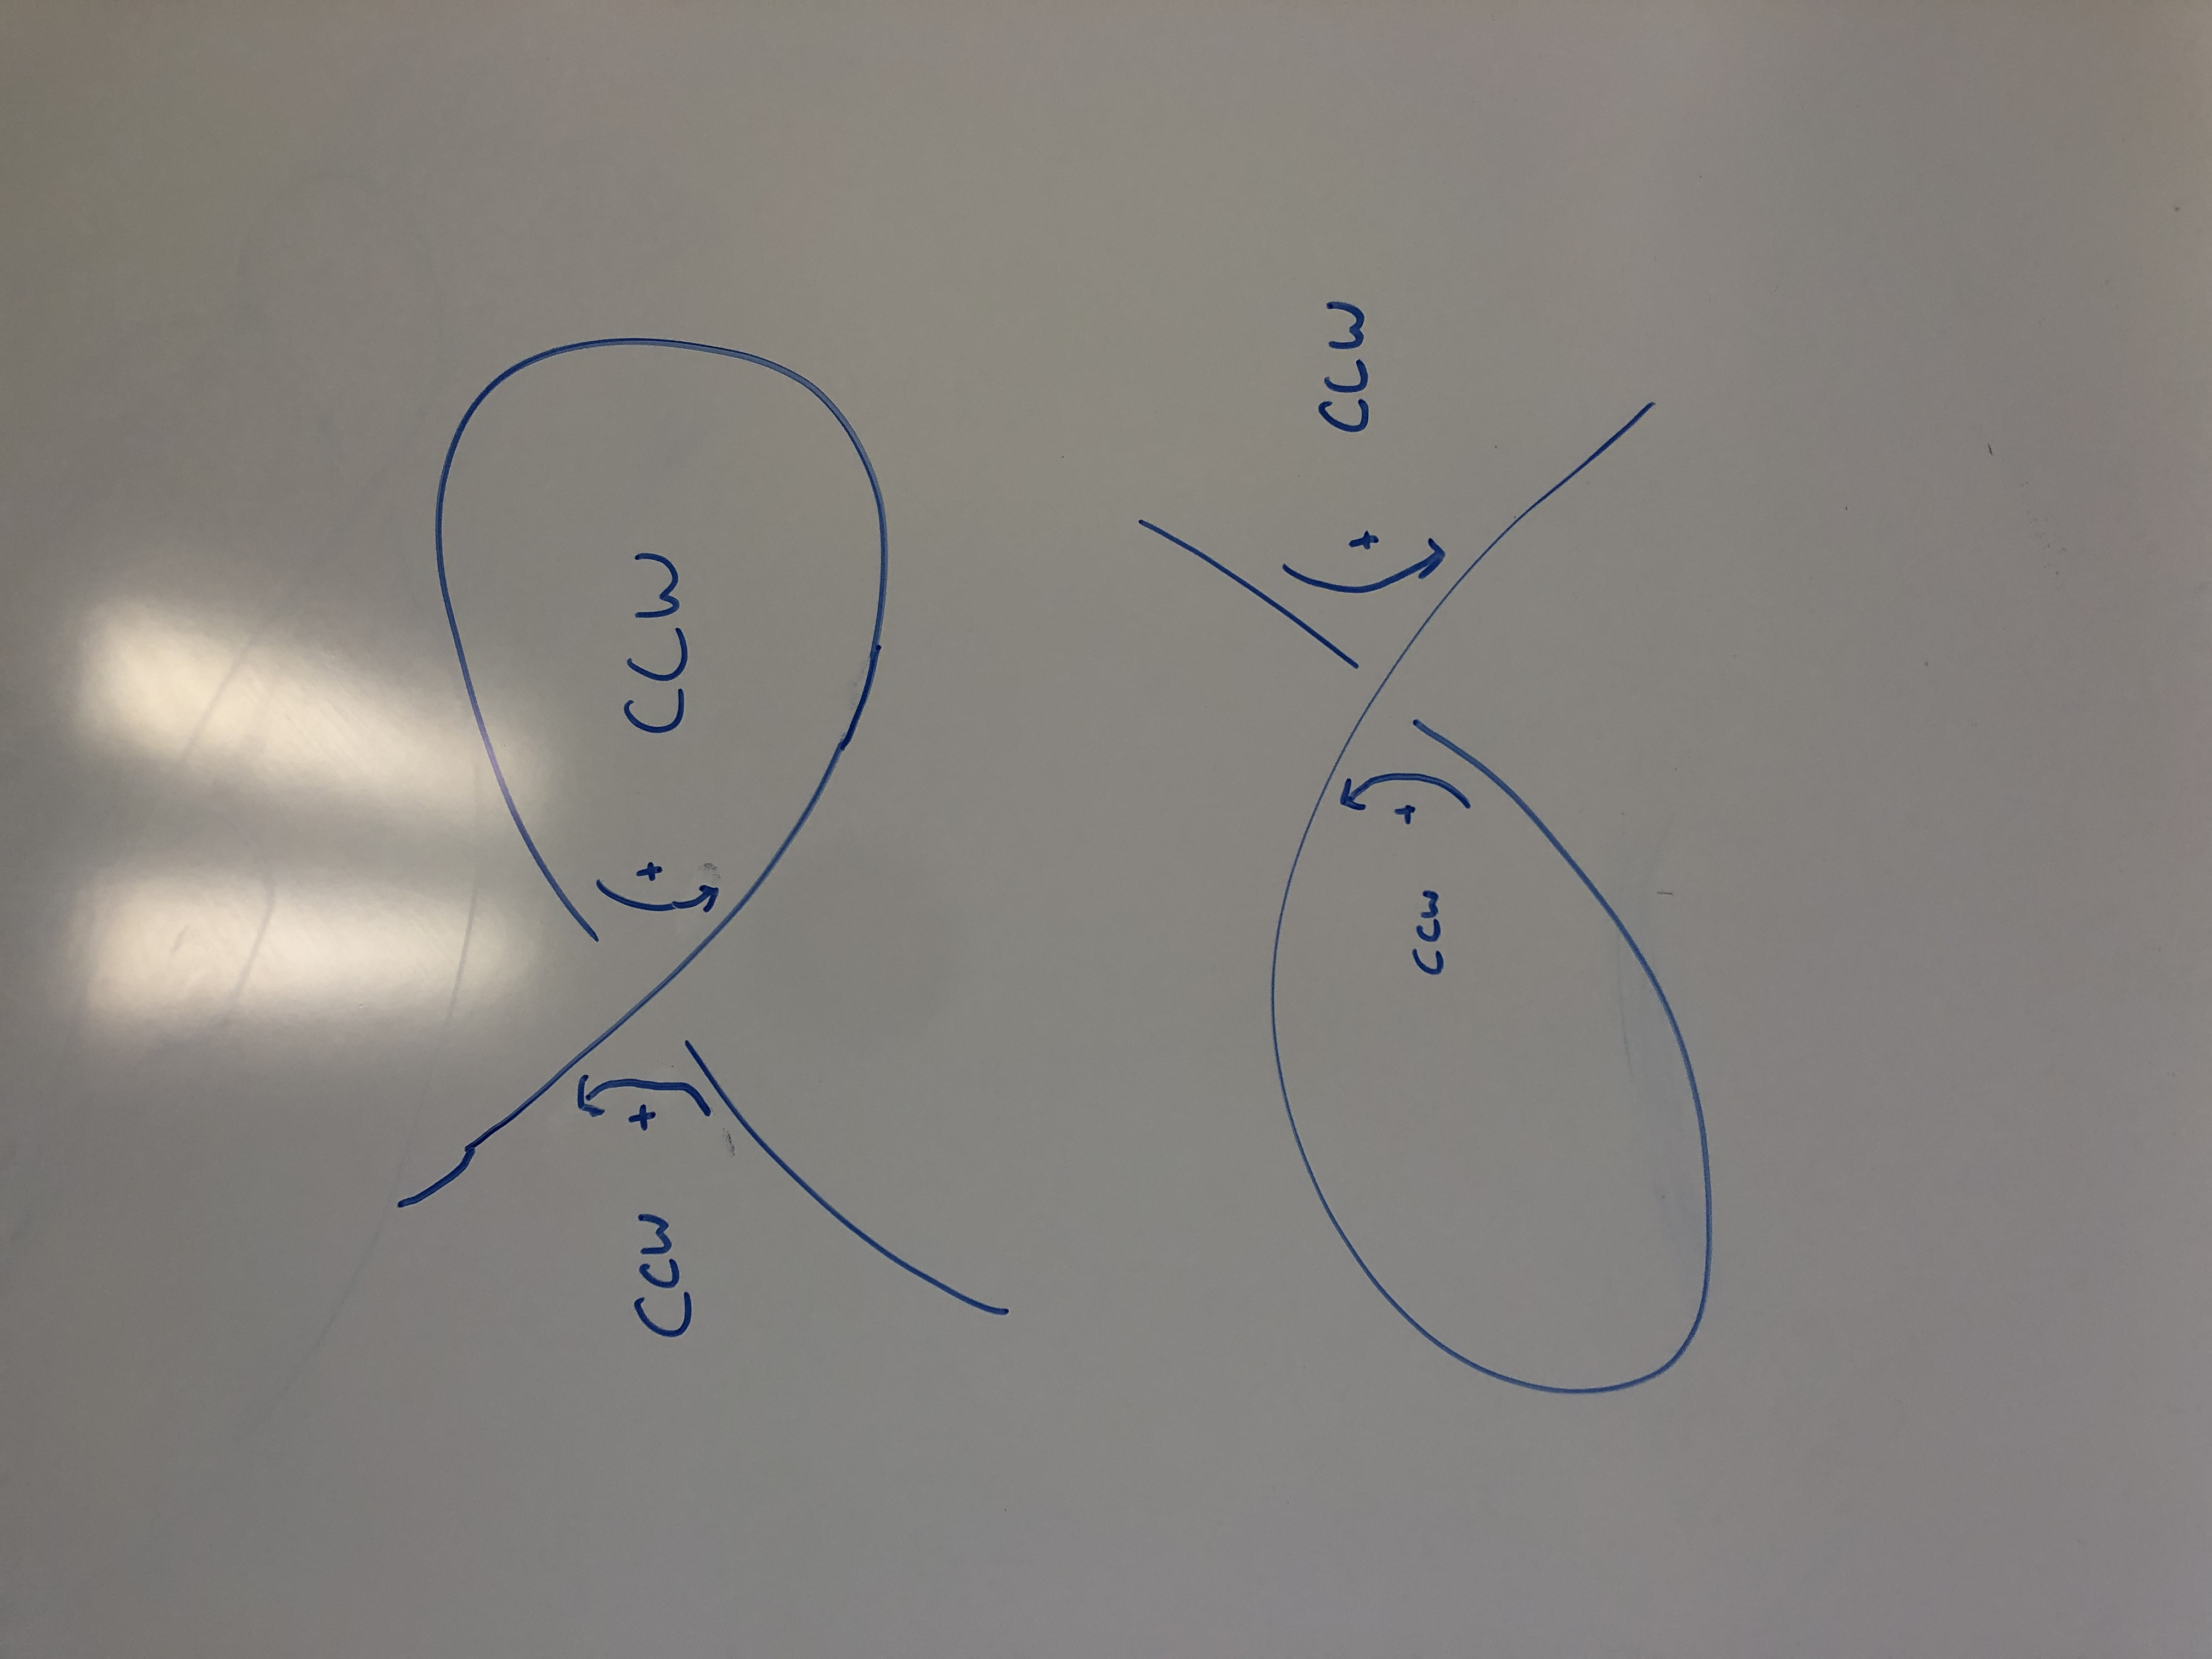
\includegraphics[width=4in,angle=-90]{Exterior Loops.JPG}



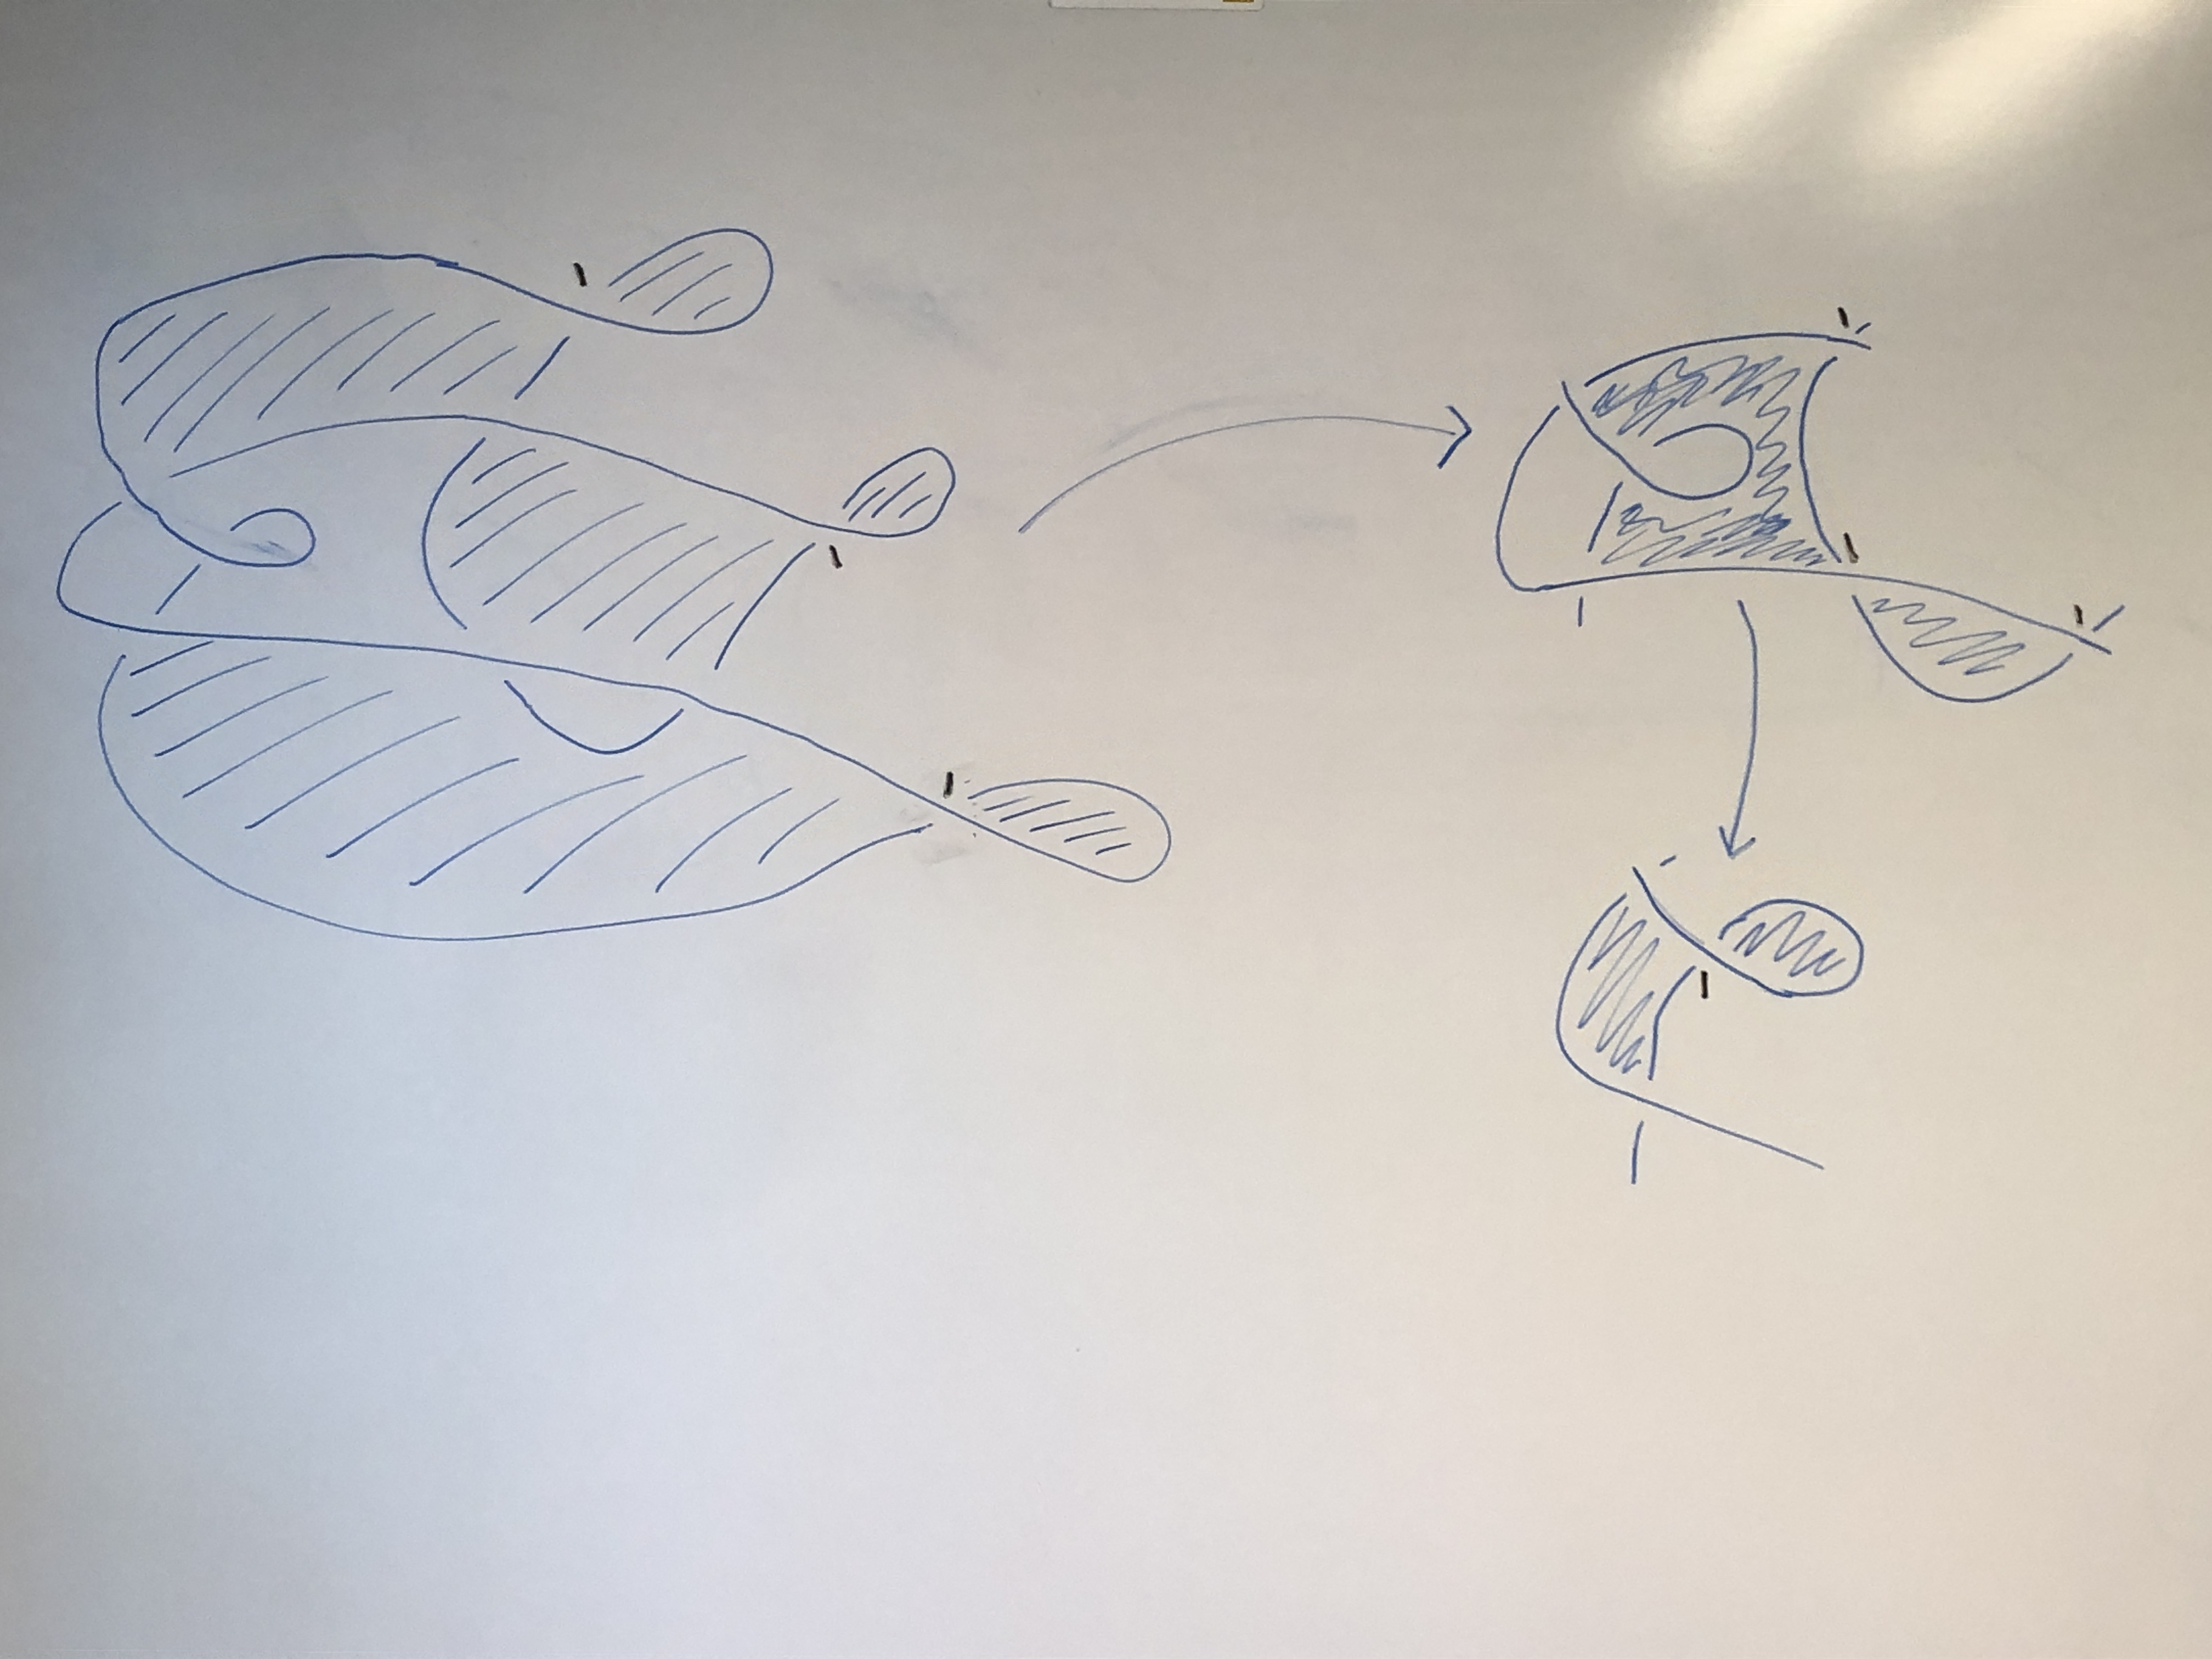
\includegraphics[width=4in]{Visualization of Algorithm.JPG}

In this manner, continue through to the nth free generators, obtaining n classes of freedom, "the extras" are class n, which are never only positive in the remaining equations
\[f^{1}_1 \cdots f^{1}_{k_1} > f^{2}_1 \cdots f^{2}_{k_2}> \cdots > f^{n-1}_1 \cdots f^{n-1}_{k_{n-1}} > k_n \text{ extras }\]

Now we work backwards - assigning those in the extras class (these are all contractible, though not all Reeb chords have to be nth free) to length 1, and then those in the $n-1$th class have length $k_n \cdot 1 + 1$ (+1 is so that we don't get exact equality) and those in the $n-2$nd class have length $ (k_n \cdot 1 + 1)\cdot k_{n-1} + 1$ and those in the $n-3$rd class $ ((k_n \cdot 1 + 1)\cdot k_{n-1} + 1)\cdot k_{n-2} + 1$ etc...




Hypothesised equivalency for height lists of the same number of generators

Perhaps an appropriate equivalency relation while include the following notion of equivalence:

Suppose that we have two classing systems of generators. Each produces many strict orderings of generators which still respect this class system. If the intersection of the set of strict orderings produced by two classing systems is nonzero, perhaps we should we consider these equivalent.




Further note:

These classes give us a filtration which is an action filtration with equities set at every opportunity. 

Examples:

add examples

Summary and further questions:

If this algorithm ends (i.e covers the entire knot) we have a way to assign heights to all of the generators. This is not unique, and is very "inefficient" in packing the values of generators closely. For example, setting those in the nth class equal to 1, we would perhaps want those in the 1st class to be as small as possible. We can do this by considering the loops one at a time backwards, setting the positive values as small as possible so that the loops are barely positive. However, if there are say two positive junctions in one of these nth loops, we no longer have uniquely determined values. 

The biggest question here is does the algorithm finish - will all areas of any loop become shaded after finite iterations (finite is guaranteed as long as the number of generators covered always increases by at least one for each class)

Additionally question, where to contractible chords show up? We know that all chords in the nth class are contractible because they are not required to be greater than any other value. However, doing the 1st Reidemiester move in the front projection and then going to the the Lagrangian projection gives us a crossing which, if the the Reidemiester moves was done along the top of a loop belonging to class 1, then now is in the second freedom class. 




\section{June 19th: Proof of algorithm in a special case}

Hand wavy thought process and motivation: 

The main issue is what happens if the algorithm doesn't finish - meaning that not all equations get crossed out. This would happen if we have inequalities involving several variables where each variable appears as both negative and positive in these inequalities. Can we come up with a counter example? It seems like trying to come up with a knot satisfying a set of inequalities with this contradiction is very difficult, if not impossible. In trying to generate valid knots I realized the difficulty was in the orientation of the crossings - because the loops can only be sideways in the Lagrangian projection (or else we have just one negative crossing in a loop). 

In trying to come up with a rigid way to quantize the knot to a grid of sorts, I realized that this already exists - plat position.

So assume that we take a knot in plat position and apply Ng's algorithm to get a knot in the lagrangian projection. Now we have something that is extremely tame and can prove that the algorithm finishes.



Lemma: The algorithm terminates and gives an ordering of heights witch satisfy the area inequalities when applied to any lagrangian projection (via Ng's algorithm) of the plat position of the front projection of a legendrian knot. 

Proof:

Consider a knot in plat position which has two types of crossings. Considering a row (we call a region such as the one shaded below a "row", a strip where it ends in a loop)



there are crossings within rows and crossings between rows. Working our way from the right






Further observations:

All extras are "super" contractable (these are generators which are never responsible for shading a loop - therefore they can \textbf{all} be set equal to zero \textbf{simultaneously}.

Not all contractible chords are super contractible - some chords may go to zero iff one of the other positive generators in their loop increases by some finite amount. 


If there are no extras (super contractible chords) than the last class are contractible, as the lack of extras implies the last set of equations to be crossed out contains no negatives. 


Contractible chords can be in classes other than the last/extras class. For example, a stabilization introduced a contractible chord in the second class.









\section{June 21st}


Algebraic description of contractability:

A contractible crossing is a generator $a_i$ in the area inequalities where for each inequality that $a_i$ appears as positive, there are no other negative terms, or if there is one or more negative terms, there is at least one other positive term.

This is a necessary condition for contractibility, but not sufficient, as if we take the "actual" definition of contractibility to be a legandrian isotopy up to the endpoint where the height goes to zero. This can not happen if the above requirement is not satisfied, however, the above requirement does not automatically guarantee the existence of such a legendrian isotopy. 


Stabilization:

Adding a stabilization with generator $a_j$ creates a contractible reed chord, because we add two things to the area inequalities: $a_j>0$ and we add a positive $a_j$ to one other area inequality. Because we previously had a valid knot, there must have been at least one other positive in this latter equation, so the added $a_j$ satisfies the necessary conditions of contractibility. 




Further Questions:



Can we list all of the possible orderings of Reeb heights?
Can we do a bunch of examples of computing FLCH?
When we have classes with multiple elements we can sometimes swap the orders. If we take the Reeb heights after swapping, how does this change FLCH (examples)?
Are finite intervals invariant under legandrian isotopy

Double shading corresponds to contractible, extras are stupid contractible (proven)


Removing a crossing and rerunning the algorithm - if the chord is contractible it should still finish

Could we prove that the algorithm finishing is preserved through isotopy by considering the equations under stable tame isomophism?

Could we use grid projection to prove things?

Make a python script to compute height assignments


Is non-switchability a property of only having two classes.


We should call this the flooding algorithm - knot is flooded  - each class is a "tier" 


Work flow:



Draw knot in plat position, get generators

Ask for z-graded differential

Compute height assignments with python

















\end{document}